% Relatorio - Controle de Temperatura de Estufa com CLP
% Jose Vitor Cardozo Amaral - UFMS
% Disciplina: Controladores Logicos Programaveis

\documentclass[
  12pt,
  openright,
  oneside,
  a4paper,
  chapter=TITLE,
  section=TITLE,
  brazilian
]{abntex2}

% Pacotes
\usepackage[utf8]{inputenc}
\usepackage[T1]{fontenc}
\usepackage{lmodern}
\usepackage{microtype}
\usepackage{indentfirst}
\usepackage{amsmath,amssymb}
\usepackage{graphicx}
\usepackage{color}
\usepackage{booktabs}
\usepackage{pdflscape}

% tira aquelas bordas vermelhas dos links no pdf
\hypersetup{hidelinks}

% Layout
\setlength{\parindent}{1.25cm}
\setlength{\parskip}{0.2cm}
\frenchspacing

% Dados do trabalho
\titulo{Controle de Temperatura de uma Estufa de Secagem para Cura de Tinta em Pe\c{c}as Met\'{a}licas Utilizando CLP}
\autor{Jos\'{e} V\'{i}tor Cardozo Amaral}
\local{Campo Grande -- MS}
\data{2025}

\orientador{Valmir Machado Pereira}
\instituicao{
  Universidade Federal de Mato Grosso do Sul -- UFMS\\
}
\renewcommand{\orientadorname}{Professor:}
\tipotrabalho{Relat\'{o}rio t\'{e}cnico}
\preambulo{Relat\'{o}rio apresentado \`{a} disciplina de Controladores L\'{o}gicos Program\'{a}veis como requisito parcial para aprova\c{c}\~{a}o, descrevendo o projeto de controle de temperatura de uma estufa de secagem para cura de tinta em pe\c{c}as met\'{a}licas utilizando CLP, com implementa\c{c}\~{o}es nos softwares LOGO!Soft Comfort (Siemens) e TPW-PCLINK (WEG).}

% Capa personalizada (ABNT)
\renewcommand{\imprimircapa}{%
  \begin{capa}%
    \center
    {\ABNTEXchapterfont\large\MakeUppercase{\imprimirinstituicao}\par}
    \vspace*{3cm}
    {\ABNTEXchapterfont\large\imprimirautor\par}
    \vfill
    {\ABNTEXchapterfont\bfseries\Large\MakeUppercase{\imprimirtitulo}\par}
    \vfill
    {\large\imprimirlocal\par}
    {\large\imprimirdata\par}
  \end{capa}%
}

% Folha de rosto
\makeatletter
\renewcommand{\folhaderostocontent}{%
  \begin{center}
    {\ABNTEXchapterfont\large\imprimirautor\par}

    \vfill

    {\ABNTEXchapterfont\bfseries\Large\MakeUppercase{\imprimirtitulo}\par}

    \vspace{2cm}

    \abntex@ifnotempty{\imprimirpreambulo}{%
      \hspace{.45\textwidth}%
      \begin{minipage}{.5\textwidth}
        \SingleSpacing
        \imprimirpreambulo\par
        \vspace{\onelineskip}
        {\imprimirorientadorRotulo~\imprimirorientador\par}
      \end{minipage}%
    }

    \vfill

    {\large\imprimirlocal\par}
    {\large\imprimirdata\par}
  \end{center}
}
\makeatother


\begin{document}
\selectlanguage{brazilian}

\pretextual

\imprimircapa
\imprimirfolhaderosto*

% Resumo
\begin{resumo}
Este relat\'{o}rio apresenta o desenvolvimento de um projeto de automa\c{c}\~{a}o para controle de temperatura de uma estufa de secagem utilizada na cura de tinta em pe\c{c}as met\'{a}licas, empregando Controladores L\'{o}gicos Program\'{a}veis (CLPs). O sistema foi implementado em duas plataformas distintas: o CLP Siemens LOGO!, programado em Diagrama de Fun\c{c}\~{o}es (FBD) no software LOGO!Soft Comfort; e o CLP WEG TPW-04, programado em Diagrama Ladder no software TPW-PCLINK.

O sistema proposto permite monitorar a temperatura interna da estufa, acionar o aquecedor de forma autom\'{a}tica por l\'{o}gica liga/desliga com histerese, realizar o tempo de cura das pe\c{c}as em uma faixa adequada de temperatura e, ao final, promover um per\'{i}odo de resfriamento controlado por um ventilador. Tamb\'{e}m foram implementadas fun\c{c}\~{o}es de seguran\c{c}a, como alarme de sobretemperatura e bloqueio de opera\c{c}\~{a}o at\'{e} o restabelecimento das condi\c{c}\~{o}es normais.

A implementa\c{c}\~{a}o dual permite comparar as abordagens de programa\c{c}\~{a}o em dois ambientes de CLPs amplamente utilizados na ind\'{u}stria, evidenciando diferen\c{c}as na forma de endere\c{c}amento, nos blocos funcionais dispon\'{i}veis e nas linguagens de programa\c{c}\~{a}o suportadas pela norma IEC~61131-3.

\textbf{Palavras-chave}: CLP; LOGO!; TPW-04; controle de temperatura; estufa de secagem; automa\c{c}\~{a}o industrial; Ladder.

\end{resumo}

\tableofcontents

\textual

%% ============================================================
\chapter{Introdu\c{c}\~{a}o}
%% ============================================================

O controle adequado de temperatura \'{e} fundamental em diversos processos industriais que envolvem secagem ou cura t\'{e}rmica de materiais. Na ind\'{u}stria de pintura de pe\c{c}as met\'{a}licas, por exemplo, \'{e} comum a utiliza\c{c}\~{a}o de estufas de secagem para garantir a cura correta da tinta, proporcionando boa ader\^{e}ncia, acabamento adequado e resist\^{e}ncia mec\^{a}nica e qu\'{i}mica ao revestimento. Quando esse processo \'{e} realizado de forma manual, com chaveamento direto do aquecedor e sem monitoramento sistem\'{a}tico da temperatura, surgem problemas como varia\c{c}\~{o}es na qualidade do produto, risco de sobreaquecimento e desperd\'{i}cio de energia el\'{e}trica.

Os Controladores L\'{o}gicos Program\'{a}veis (CLPs) s\~{a}o dispositivos largamente empregados na automa\c{c}\~{a}o industrial para substitui\c{c}\~{a}o de pain\'{e}is de rel\'{e}s e implementa\c{c}\~{a}o de l\'{o}gicas de controle de forma flex\'{i}vel, confi\'{a}vel e facilmente reprogram\'{a}vel. Atualmente, existem diversos fabricantes e fam\'{i}lias de CLPs dispon\'{i}veis no mercado, cada qual com caracter\'{i}sticas pr\'{o}prias de hardware, ambiente de programa\c{c}\~{a}o e linguagens suportadas. A norma IEC~61131-3 define cinco linguagens padr\~{a}o para programa\c{c}\~{a}o de CLPs: Diagrama Ladder (LD), Texto Estruturado (ST), Diagrama de Blocos Funcionais (FBD), Gr\'{a}fico de Fun\c{c}\~{o}es Sequenciais (SFC), entre outras.

Neste trabalho, \'{e} desenvolvido um sistema de controle de temperatura para uma estufa de secagem de pe\c{c}as met\'{a}licas pintadas, implementado em \textbf{duas plataformas de CLP distintas}:
\begin{itemize}
    \item \textbf{Siemens LOGO!}, programado em Diagrama de Blocos Funcionais (FBD) no software LOGO!Soft Comfort;
    \item \textbf{WEG TPW-04}, programado em Diagrama Ladder no software TPW-PCLINK V1.12.
\end{itemize}

A implementa\c{c}\~{a}o dual permite ao estudante e ao leitor comparar como o mesmo algoritmo de controle pode ser traduzido para ambientes de programa\c{c}\~{a}o e conjuntos de instru\c{c}\~{o}es diferentes, evidenciando as particularidades de cada plataforma e refor\c{c}ando o dom\'{i}nio dos conceitos fundamentais de programa\c{c}\~{a}o de CLPs.

%% ============================================================
\chapter{Objetivos}
%% ============================================================

\section{Objetivo geral}

O objetivo geral deste trabalho \'{e} desenvolver um sistema de automa\c{c}\~{a}o, baseado em CLP, para o controle de temperatura de uma estufa de secagem utilizada na cura de tinta em pe\c{c}as met\'{a}licas, implementando o mesmo algoritmo de controle em duas plataformas distintas --- Siemens LOGO! e WEG TPW-04 --- utilizando recursos de entrada e sa\'{i}da anal\'{o}gicas, comparadores, temporizadores, intertravamentos e diferentes linguagens de programa\c{c}\~{a}o de CLPs.

\section{Objetivos espec\'{i}ficos}

Como objetivos espec\'{i}ficos, destacam-se:
\begin{itemize}
    \item Especificar o processo de secagem e os requisitos de temperatura e tempo de cura para as pe\c{c}as met\'{a}licas pintadas;
    \item Definir e mapear as entradas e sa\'{i}das digitais e anal\'{o}gicas do CLP necess\'{a}rias para o controle do processo;
    \item Implementar, em ambiente LOGO!Soft Comfort, um programa de controle em FBD que:
    \begin{itemize}
        \item leia a temperatura da estufa por meio de uma entrada anal\'{o}gica;
        \item trate o sinal com amplificador anal\'{o}gico, estabelecendo escala em graus Celsius (\textdegree{}C);
        \item utilize comparadores anal\'{o}gicos para definir faixas de opera\c{c}\~{a}o, in\'{i}cio de cura e sobretemperatura;
        \item acione o aquecedor de forma autom\'{a}tica, com l\'{o}gica liga/desliga e histerese de temperatura;
        \item realize o tempo de cura em faixa adequada de temperatura por meio de temporizadores;
        \item realize o resfriamento ap\'{o}s a cura por um per\'{i}odo determinado, acionando um ventilador;
        \item gere alarmes e intertravamentos em caso de sobretemperatura e porta aberta;
    \end{itemize}
    \item Implementar o mesmo algoritmo de controle no CLP WEG TPW-04, utilizando Diagrama Ladder no software TPW-PCLINK;
    \item Comparar as duas implementa\c{c}\~{o}es, destacando diferen\c{c}as de endere\c{c}amento, blocos funcionais e abordagem de programa\c{c}\~{a}o;
    \item Implementar uma interface simples no display do CLP LOGO!, exibindo temperatura atual e estado do processo.
\end{itemize}

%% ============================================================
\chapter{Fundamenta\c{c}\~{a}o te\'{o}rica}
%% ============================================================

\section{Controladores L\'{o}gicos Program\'{a}veis}

Controladores L\'{o}gicos Program\'{a}veis (CLPs) s\~{a}o equipamentos microprocessados desenvolvidos para automa\c{c}\~{a}o de processos industriais, substituindo circuitos fixos de rel\'{e}s e permitindo a implementa\c{c}\~{a}o de l\'{o}gicas de controle por meio de programas. Um CLP t\'{i}pico apresenta entradas e sa\'{i}das digitais, m\'{o}dulos anal\'{o}gicos opcionais, mem\'{o}ria n\~{a}o vol\'{a}til para armazenamento do programa e recursos de comunica\c{c}\~{a}o com outros dispositivos.

Entre as vantagens dos CLPs em rela\c{c}\~{a}o a circuitos baseados em rel\'{e}s, destacam-se a facilidade de reprograma\c{c}\~{a}o, maior confiabilidade, capacidade de diagn\'{o}stico e manuten\c{c}\~{a}o, possibilidade de expans\~{a}o modular e integra\c{c}\~{a}o com sistemas de supervis\~{a}o e controle. Em aplica\c{c}\~{o}es envolvendo vari\'{a}veis de processo cont\'{i}nuas (como temperatura, n\'{i}vel ou press\~{a}o), s\~{a}o empregados m\'{o}dulos de entrada e sa\'{i}da anal\'{o}gicas.

\section{O CLP Siemens LOGO!}

A fam\'{i}lia LOGO!, da Siemens, \'{e} uma linha de micro-CLPs compactos amplamente utilizados em aplica\c{c}\~{o}es de automa\c{c}\~{a}o predial e industrial de pequeno porte. Os modelos da fam\'{i}lia LOGO! possuem entradas e sa\'{i}das digitais integradas, al\'{e}m de vers\~{o}es com entradas e sa\'{i}das anal\'{o}gicas embutidas. O software de programa\c{c}\~{a}o LOGO!Soft Comfort permite a cria\c{c}\~{a}o de programas em Diagrama de Blocos Funcionais (FBD), oferecendo blocos como temporizadores, comparadores anal\'{o}gicos, amplificadores anal\'{o}gicos, mem\'{o}rias RS e blocos de mensagem para o display integrado.

O LOGO! possui display e teclas de opera\c{c}\~{a}o integrados, permitindo a implementa\c{c}\~{a}o de interfaces homem--m\'{a}quina (IHM) simples diretamente no controlador, sem necessidade de equipamentos adicionais.

\section{O CLP WEG TPW-04}

A fam\'{i}lia TPW-04, fabricada pela WEG, \'{e} uma linha de micro-CLPs voltada para aplica\c{c}\~{o}es industriais. O modelo TPW04-114BR-A possui 8 entradas digitais e 6 sa\'{i}das a rel\'{e}, com endere\c{c}amento octal para entradas (X) e sa\'{i}das (Y), e capacidade de expans\~{a}o com m\'{o}dulos anal\'{o}gicos.

O software de programa\c{c}\~{a}o TPW-PCLINK V1.12 suporta a linguagem \textbf{Diagrama Ladder (LD)} da norma IEC~61131-3, permitindo ao programador construir a l\'{o}gica de controle de forma gr\'{a}fica, utilizando contatos, bobinas e blocos de fun\c{c}\~{a}o organizados em \textit{rungs} (degraus).

Entre os recursos dispon\'{i}veis no TPW-04 est\~{a}o: temporizadores com diversas bases de tempo (1~ms, 10~ms e 100~ms), contadores de 16 e 32 bits, contatos de compara\c{c}\~{a}o no diagrama Ladder para avalia\c{c}\~{a}o de registradores, blocos de fun\c{c}\~{o}es aritm\'{e}ticas (soma, subtra\c{c}\~{a}o, multiplica\c{c}\~{a}o, divis\~{a}o), controle PID integrado (FNC~88), comunica\c{c}\~{a}o serial e MODBUS, al\'{e}m de at\'{e} 8000 passos de programa.

\section{Linguagens de programa\c{c}\~{a}o de CLPs (IEC~61131-3)}

A norma IEC~61131-3 padroniza cinco linguagens para programa\c{c}\~{a}o de CLPs. Neste trabalho s\~{a}o utilizadas duas delas:

\begin{itemize}
    \item \textbf{Diagrama de Blocos Funcionais (FBD)}: linguagem gr\'{a}fica na qual o programa \'{e} constru\'{i}do pela conex\~{a}o de blocos funcionais (portas l\'{o}gicas, temporizadores, comparadores etc.) por meio de linhas de sinal. Utilizada no LOGO!Soft Comfort.
    \item \textbf{Diagrama Ladder (LD)}: linguagem gr\'{a}fica baseada na representa\c{c}\~{a}o de circuitos el\'{e}tricos a rel\'{e}s, com contatos (entradas) e bobinas (sa\'{i}das) organizados em degraus (\textit{rungs}). Utilizada no TPW-PCLINK.
\end{itemize}

\section{Sinais anal\'{o}gicos de entrada e sa\'{i}da}

Sinais anal\'{o}gicos s\~{a}o aqueles que variam de forma cont\'{i}nua dentro de uma determinada faixa e geralmente s\~{a}o representados, em automa\c{c}\~{a}o industrial, por correntes padronizadas (4--20~mA) ou tens\~{o}es (0--10~V). Sensores de temperatura, como termorresist\^{e}ncias (PT100) ou termopares, s\~{a}o frequentemente associados a transmissores que convertem a grandeza medida em um sinal anal\'{o}gico el\'{e}trico compat\'{i}vel com a entrada do CLP.

Nas entradas anal\'{o}gicas do CLP, o valor f\'{i}sico medido \'{e} convertido por um conversor anal\'{o}gico--digital (ADC) em um n\'{u}mero inteiro proporcional \`{a} grandeza. No LOGO!, a entrada anal\'{o}gica gera valores de 0 a 1000 internamente. No TPW-04, a leitura anal\'{o}gica \'{e} armazenada em registradores de dados especiais (D8436 em diante), e a instru\c{c}\~{a}o EPSC (FNC~89) permite a escala autom\'{a}tica do valor lido. Alternativamente, os potenci\^{o}metros internos do TPW-04 (VR0 e VR1, lidos pela instru\c{c}\~{a}o VRRD -- FNC~85) podem ser utilizados para simula\c{c}\~{a}o de sinais anal\'{o}gicos, gerando valores de 0 a 1023.

\section{Comparadores e amplificadores anal\'{o}gicos}

No LOGO!, blocos de \textit{amplificador anal\'{o}gico} aplicam ganho e deslocamento (\textit{offset}) a um valor de entrada, permitindo a convers\~{a}o de escalas. Blocos de \textit{comparador anal\'{o}gico} geram sinais digitais a partir de compara\c{c}\~{o}es com limiares, possibilitando a implementa\c{c}\~{a}o de l\'{o}gicas de histerese.

No TPW-04, a mesma funcionalidade \'{e} obtida por meio de blocos de fun\c{c}\~{o}es aritm\'{e}ticas (MUL, DIV) para escala, e contatos de compara\c{c}\~{a}o no diagrama Ladder para detec\c{c}\~{a}o de faixas de opera\c{c}\~{a}o. Esses contatos comparam diretamente registradores de dados com constantes ou outros registradores, sem necessidade de blocos dedicados.

\section{Controle liga/desliga com histerese}

O controle liga/desliga \'{e} uma forma simples de controle que aciona um atuador quando a vari\'{a}vel de processo est\'{a} abaixo (ou acima) de um valor de refer\^{e}ncia e o desliga quando atinge outro limite. Para evitar comuta\c{c}\~{o}es muito r\'{a}pidas em torno de um \'{u}nico ponto, \'{e} habitual se trabalhar com histerese, definindo uma faixa de opera\c{c}\~{a}o.

No contexto deste trabalho, o aquecedor da estufa \'{e} comandado por uma l\'{o}gica liga/desliga com histerese de temperatura: o aquecedor \'{e} ligado quando a temperatura est\'{a} abaixo de 115~\textdegree{}C e desligado quando ultrapassa 125~\textdegree{}C. Dessa forma, a temperatura oscila dentro de uma faixa de 10~\textdegree{}C em torno do valor de \textit{setpoint} de 120~\textdegree{}C. Em ambos os CLPs, essa l\'{o}gica \'{e} implementada por meio de mem\'{o}rias de reten\c{c}\~{a}o (RS no LOGO!; SET/RST no TPW-04) combinadas com compara\c{c}\~{o}es anal\'{o}gicas.

\section{Temporizadores e l\'{o}gica de seguran\c{c}a}

Temporizadores s\~{a}o blocos fundamentais em CLPs e permitem implementar atrasos na energiza\c{c}\~{a}o de sa\'{i}das ou contagens de tempo em regime. No LOGO!, s\~{a}o utilizados blocos de temporiza\c{c}\~{a}o do tipo \textit{on-delay}. No TPW-04, os temporizadores T0--T199 operam com base de tempo de 100~ms, sendo ativados por bobinas de temporizador nos respectivos \textit{rungs} do diagrama Ladder, com valor de \textit{setpoint} definido como constante.

Neste projeto, s\~{a}o utilizados dois temporizadores: um para o tempo de cura (30 minutos em opera\c{c}\~{a}o real; 10 segundos para demonstra\c{c}\~{a}o) e outro para o tempo de resfriamento (5 minutos em opera\c{c}\~{a}o real; 7 segundos para demonstra\c{c}\~{a}o). Al\'{e}m disso, s\~{a}o implementadas l\'{o}gicas de seguran\c{c}a com alarmes e intertravamentos para sobretemperatura e verifica\c{c}\~{a}o de porta.

%% ============================================================
\chapter{Modo de abordagem utilizado}
%% ============================================================

A abordagem adotada para o desenvolvimento do controle proposto seguiu as etapas descritas a seguir.

\section{Defini\c{c}\~{a}o do processo e requisitos}

Inicialmente foi definido o processo f\'{i}sico a ser automatizado: uma estufa de secagem utilizada para cura de tinta l\'{i}quida aplicada em pe\c{c}as met\'{a}licas. Com base em dados t\'{i}picos de processos de pintura, foram estabelecidos valores de refer\^{e}ncia para o projeto:

\begin{itemize}
    \item Temperatura de \textit{setpoint} para cura: aproximadamente 120~\textdegree{}C;
    \item Faixa de cura considerada adequada: 115~\textdegree{}C a 125~\textdegree{}C;
    \item Temperatura de seguran\c{c}a (sobreaquecimento): 150~\textdegree{}C;
    \item Tempo m\'{i}nimo de cura dentro da faixa de temperatura: 30 minutos (utilizou-se 10 segundos para demonstra\c{c}\~{a}o);
    \item Tempo de resfriamento ap\'{o}s a cura, com ventila\c{c}\~{a}o: 5 minutos (utilizou-se 7 segundos para demonstra\c{c}\~{a}o).
\end{itemize}

Tamb\'{e}m foram definidas as condi\c{c}\~{o}es de opera\c{c}\~{a}o: o processo \'{e} iniciado pelo operador por meio de um bot\~{a}o de \textit{Start}, com intertravamento de porta fechada, e deve ser automaticamente interrompido em caso de sobretemperatura ou abertura da porta.

\section{Especifica\c{c}\~{a}o do CLP e das vari\'{a}veis de entrada e sa\'{i}da}

Foram especificados dois CLPs para implementa\c{c}\~{a}o do mesmo algoritmo de controle:
\begin{itemize}
    \item \textbf{Siemens LOGO! 12/24RCE}: com 8 entradas digitais, 4 sa\'{i}das a rel\'{e}, entradas e sa\'{i}das anal\'{o}gicas integradas, e display com teclas para IHM;
    \item \textbf{WEG TPW04-114BR-A}: com 8 entradas digitais, 6 sa\'{i}das a rel\'{e} e possibilidade de expans\~{a}o anal\'{o}gica.
\end{itemize}

\section{Modelagem do algoritmo de controle}

Em seguida, foi elaborado o algoritmo de controle do processo, \'{u}nico para ambas as plataformas. O algoritmo contempla as seguintes fun\c{c}\~{o}es principais:

\begin{itemize}
    \item partida e parada do sistema, com mem\'{o}ria de opera\c{c}\~{a}o;
    \item leitura da temperatura, tratamento do sinal e compara\c{c}\~{a}o com limites de opera\c{c}\~{a}o;
    \item comando do aquecedor com histerese de temperatura;
    \item temporiza\c{c}\~{a}o do tempo de cura na faixa de temperatura;
    \item temporiza\c{c}\~{a}o do resfriamento com ventilador;
    \item tratamento de alarmes e intertravamentos de seguran\c{c}a;
    \item atualiza\c{c}\~{a}o das mensagens de IHM (apenas no LOGO!, que possui display integrado).
\end{itemize}

\section{Implementa\c{c}\~{a}o em dois ambientes de programa\c{c}\~{a}o}

Com o algoritmo definido, o programa foi implementado em dois ambientes:
\begin{enumerate}
    \item No \textbf{LOGO!Soft Comfort}, utilizando Diagrama de Blocos Funcionais (FBD) com blocos de mem\'{o}ria RS, comparadores anal\'{o}gicos, amplificadores anal\'{o}gicos, temporizadores \textit{on-delay}, portas l\'{o}gicas e blocos de mensagem de texto para o display.
    \item No \textbf{TPW-PCLINK V1.12}, utilizando Diagrama Ladder, com contatos normalmente abertos e fechados, bobinas de sa\'{i}da, bobinas SET/RST, contatos de compara\c{c}\~{a}o, blocos de fun\c{c}\~{o}es aritm\'{e}ticas (MOV, DIV) e temporizadores T0--T1.
\end{enumerate}

\section{Valida\c{c}\~{a}o em simula\c{c}\~{a}o}

Ambos os programas foram validados em simula\c{c}\~{a}o nos respectivos softwares, observando-se o comportamento das sa\'{i}das digitais diante de diferentes condi\c{c}\~{o}es de temperatura e comandos do operador. A simula\c{c}\~{a}o permitiu verificar o funcionamento correto das l\'{o}gicas de aquecimento, cura, resfriamento e alarme.

%% ============================================================
\chapter{Desenvolvimento te\'{o}rico e pr\'{a}tico}
%% ============================================================

\section{Descri\c{c}\~{a}o do processo f\'{i}sico}

O processo considerado \'{e} a cura de tinta l\'{i}quida aplicada em pe\c{c}as met\'{a}licas, realizada em uma estufa de secagem. Ap\'{o}s a pintura, as pe\c{c}as s\~{a}o colocadas no interior da estufa, a porta \'{e} fechada e o operador aciona o sistema por meio de um bot\~{a}o de \textit{Start}. O aquecedor \'{e} ent\~{a}o acionado, elevando a temperatura interna at\'{e} a faixa adequada para cura (em torno de 120~\textdegree{}C).

Uma vez atingida essa faixa, as pe\c{c}as devem permanecer na estufa por um tempo m\'{i}nimo de 30 minutos para garantir a cura completa da tinta. Ap\'{o}s a conclus\~{a}o do tempo de cura, o aquecedor \'{e} desligado e um ventilador interno \'{e} acionado por 5 minutos para promover o resfriamento controlado do ambiente. Ao final, a estufa retorna ao estado de espera, permitindo a retirada das pe\c{c}as pelo operador.

Para garantir seguran\c{c}a, foram definidos mecanismos de prote\c{c}\~{a}o: em caso de sobretemperatura (T $>$ 150~\textdegree{}C), o aquecedor \'{e} desligado imediatamente, um alarme \'{e} acionado e o sistema n\~{a}o pode ser reiniciado at\'{e} que a temperatura retorne a um valor seguro e o operador realize o \textit{reset} do alarme. Adicionalmente, a abertura da porta durante a opera\c{c}\~{a}o provoca o desligamento imediato do aquecedor.

\section{Especifica\c{c}\~{a}o de entradas e sa\'{i}das}

A Tabela~\ref{tab:io_logo} apresenta o mapeamento de entradas e sa\'{i}das para o CLP Siemens LOGO!, e a Tabela~\ref{tab:io_tpw} apresenta o mapeamento equivalente para o CLP WEG TPW-04.

\begin{table}[htbp]
\centering
\caption{Mapeamento de entradas e sa\'{i}das -- Siemens LOGO!}
\label{tab:io_logo}
\begin{tabular}{llp{7.5cm}}
\toprule
\textbf{Endere\c{c}o} & \textbf{Tipo} & \textbf{Descri\c{c}\~{a}o} \\
\midrule
I1   & Entrada digital  & Bot\~{a}o \textit{Start} (partida do sistema) \\
I2   & Entrada digital  & Bot\~{a}o \textit{Stop} (parada do sistema) \\
I3   & Entrada digital  & Contato de porta fechada da estufa \\
I4   & Entrada digital  & Bot\~{a}o \textit{Reset} de alarme \\
AI1  & Entrada anal\'{o}gica & Sensor de temperatura (0--10~V) \\
Q1   & Sa\'{i}da digital    & Contator do aquecedor \\
Q2   & Sa\'{i}da digital    & Ventilador interno (resfriamento) \\
Q3   & Sa\'{i}da digital    & L\^{a}mpada ``em opera\c{c}\~{a}o'' \\
Q4   & Sa\'{i}da digital    & Alarme de sobretemperatura \\
Q5   & Sa\'{i}da digital    & L\^{a}mpada ``processo conclu\'{i}do'' \\
AQ1  & Sa\'{i}da anal\'{o}gica  & Sinal 0--10~V proporcional \`{a} temperatura \\
\bottomrule
\end{tabular}
\end{table}

\begin{table}[htbp]
\centering
\caption{Mapeamento de entradas e sa\'{i}das -- WEG TPW-04.}
\label{tab:io_tpw}
\begin{tabular}{llp{7.5cm}}
\toprule
\textbf{Endere\c{c}o} & \textbf{Tipo} & \textbf{Descri\c{c}\~{a}o} \\
\midrule
X000 & Entrada digital  & Bot\~{a}o \textit{Start} (partida do sistema) \\
X001 & Entrada digital  & Bot\~{a}o \textit{Stop} (parada do sistema) \\
X002 & Entrada digital  & Contato de porta fechada da estufa \\
X003 & Entrada digital  & Bot\~{a}o \textit{Reset} de alarme \\
Y000 & Sa\'{i}da digital    & Contator do aquecedor \\
Y001 & Sa\'{i}da digital    & Ventilador interno (resfriamento) \\
Y002 & Sa\'{i}da digital    & L\^{a}mpada ``em opera\c{c}\~{a}o'' \\
Y003 & Sa\'{i}da digital    & Alarme de sobretemperatura \\
Y004 & Sa\'{i}da digital    & L\^{a}mpada ``processo conclu\'{i}do'' \\
\midrule
M0   & Mem\'{o}ria interna   & Estado do sistema (RUN) \\
M1   & Mem\'{o}ria interna   & Alarme ativo \\
M2   & Mem\'{o}ria interna   & Aquecedor habilitado \\
M3   & Mem\'{o}ria interna   & Cura finalizada \\
M4   & Mem\'{o}ria interna   & Resfriamento completo \\
D0   & Registrador       & Leitura bruta do potenci\^{o}metro (0--1023) \\
D1   & Registrador       & Temperatura em \textdegree{}C (0--204) \\
T0   & Temporizador      & Timer de cura (base 100~ms) \\
T1   & Temporizador      & Timer de resfriamento (base 100~ms) \\
\bottomrule
\end{tabular}
\end{table}

\section{Algoritmo de controle}

O algoritmo de controle, comum a ambas as implementa\c{c}\~{o}es, pode ser resumido nas seguintes etapas:

\begin{enumerate}
    \item Verificar se a porta da estufa est\'{a} fechada e se n\~{a}o h\'{a} alarme ativo. Se estas condi\c{c}\~{o}es forem atendidas e o operador pressionar o bot\~{a}o \textit{Start}, o sistema entra em opera\c{c}\~{a}o (\textit{RUN}).
    \item Em modo \textit{RUN}, a temperatura da estufa \'{e} continuamente lida e convertida em graus Celsius.
    \item Enquanto a temperatura estiver abaixo de 115~\textdegree{}C, o aquecedor \'{e} acionado. Quando a temperatura atinge 125~\textdegree{}C, o aquecedor \'{e} desligado (histerese de 10~\textdegree{}C).
    \item Quando a temperatura atinge a faixa de cura (acima de 115~\textdegree{}C) e o sistema est\'{a} em opera\c{c}\~{a}o, \'{e} acionado um temporizador de 30 minutos.
    \item Ao final dos 30 minutos de cura, o aquecedor \'{e} definitivamente bloqueado e \'{e} acionado um temporizador de 5 minutos de resfriamento, que mant\'{e}m o ventilador interno ligado.
    \item Ao t\'{e}rmino do tempo de resfriamento, o ventilador \'{e} desligado e o sistema retorna ao estado de espera, acendendo a indica\c{c}\~{a}o de processo conclu\'{i}do.
    \item Em qualquer momento, caso a temperatura ultrapasse 150~\textdegree{}C, o sistema desliga o aquecedor, aciona o alarme e impede nova partida at\'{e} que a temperatura retorne abaixo de 130~\textdegree{}C e o operador pressione o bot\~{a}o de \textit{Reset}.
    \item A abertura da porta durante a opera\c{c}\~{a}o tamb\'{e}m provoca a parada do sistema.
\end{enumerate}

\section{Implementa\c{c}\~{a}o no LOGO!Soft Comfort (Siemens)}

O programa foi organizado em redes l\'{o}gicas (\textit{networks}) no LOGO!Soft Comfort, cada uma com uma fun\c{c}\~{a}o espec\'{i}fica. A seguir \'{e} apresentada uma descri\c{c}\~{a}o das principais redes:

\begin{itemize}
    \item \textbf{Rede de partida/parada (RUN)}: implementa uma mem\'{o}ria RS que representa o estado de ``sistema em opera\c{c}\~{a}o''. A entrada \textit{Set} \'{e} acionada pelo bot\~{a}o \textit{Start} (I1), desde que a porta esteja fechada (I3) e n\~{a}o haja alarme. A entrada \textit{Reset} \'{e} acionada pelo bot\~{a}o \textit{Stop} (I2), pela abertura da porta ou pela ativa\c{c}\~{a}o de alarme. A mem\'{o}ria RUN comanda a sa\'{i}da Q3.
    \item \textbf{Rede de tratamento anal\'{o}gico}: l\^{e} a entrada anal\'{o}gica AI1 e a converte em temperatura em graus Celsius por meio de um bloco amplificador anal\'{o}gico (ganho de 0,2 e offset zero, convertendo a faixa 0--1000 para 0--200~\textdegree{}C). A sa\'{i}da deste bloco \'{e} utilizada em comparadores anal\'{o}gicos e tamb\'{e}m \'{e} reenviada, ap\'{o}s ajuste de escala (ganho de 0,05), \`{a} sa\'{i}da anal\'{o}gica AQ1 para monitoramento.
    \item \textbf{Rede de alarme de sobretemperatura}: utiliza um comparador anal\'{o}gico configurado com limiares de 150~\textdegree{}C (ligar alarme) e 130~\textdegree{}C (desligar), gerando um sinal digital que aciona a sa\'{i}da Q4 e bloqueia o sistema.
    \item \textbf{Rede de controle do aquecedor}: implementa o controle liga/desliga com histerese por meio de dois comparadores anal\'{o}gicos (115~\textdegree{}C e 125~\textdegree{}C) e uma mem\'{o}ria RS que comanda a sa\'{i}da Q1.
    \item \textbf{Rede de temporiza\c{c}\~{a}o de cura}: detecta quando a temperatura est\'{a} na faixa de cura e aciona um temporizador \textit{on-delay}. Ao t\'{e}rmino, registra a condi\c{c}\~{a}o de ``cura finalizada'' e bloqueia o aquecedor.
    \item \textbf{Rede de resfriamento}: ap\'{o}s a cura, um segundo temporizador comanda o ventilador (Q2) e, ao expirar, retorna o sistema ao estado de espera e aciona a indica\c{c}\~{a}o de processo conclu\'{i}do (Q5).
    \item \textbf{Rede da IHM}: blocos de mensagem de texto exibem telas no display com temperatura atual e mensagens de estado.
\end{itemize}

A Figura~\ref{fig:clp_geral} apresenta a vis\~{a}o geral do programa desenvolvido no LOGO!Soft Comfort.

\begin{figure}[htbp]
\centering
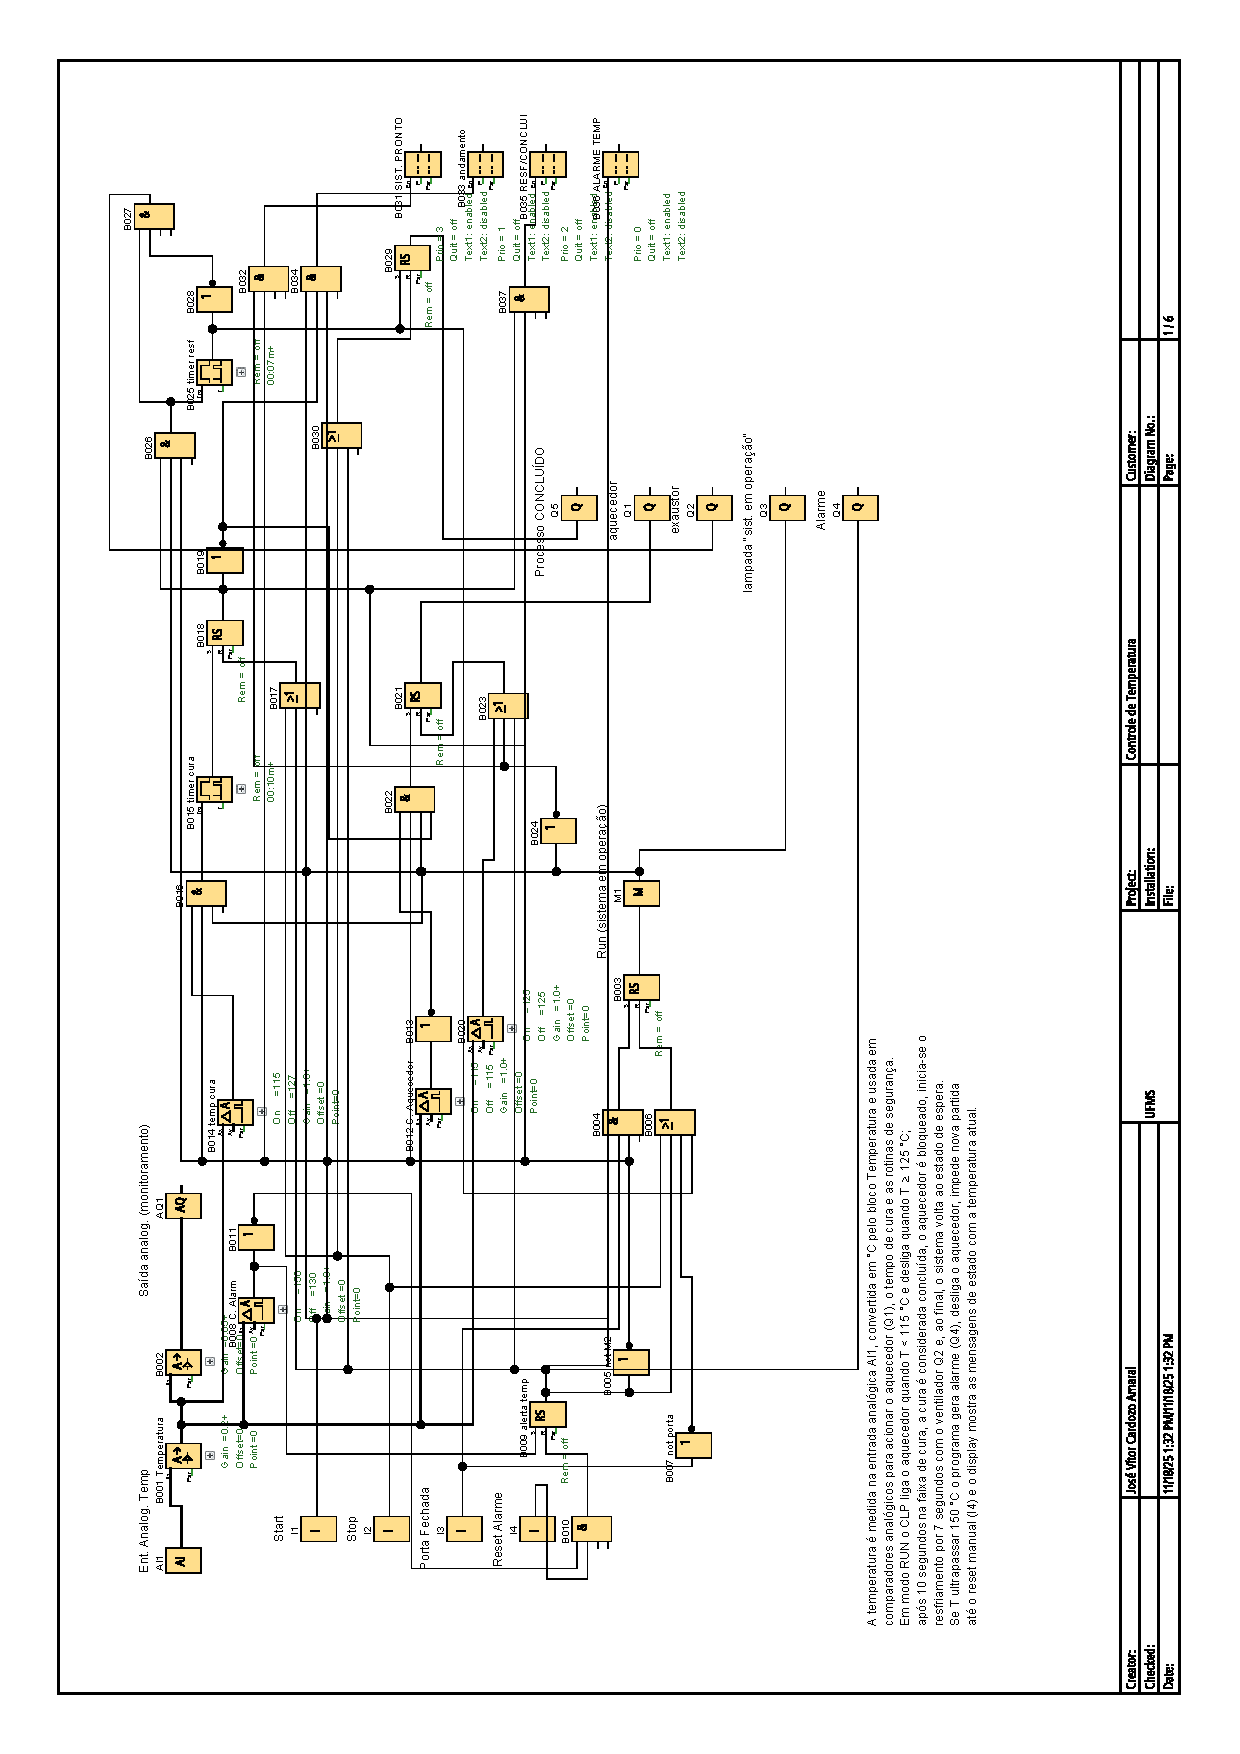
\includegraphics[angle=270,width=1\textwidth]{clp.pdf}
\caption{Vis\~{a}o geral do projeto desenvolvido no LOGO!Soft Comfort (FBD).}
\label{fig:clp_geral}
\end{figure}

\clearpage

\subsection{Interface homem--m\'{a}quina (IHM) no LOGO!}

A IHM foi implementada no pr\'{o}prio display do CLP LOGO!, utilizando blocos de texto configurados para exibir mensagens conforme estados l\'{o}gicos do programa:

\begin{itemize}
    \item \textbf{Sistema pronto}: exibida quando o sistema n\~{a}o est\'{a} em RUN e n\~{a}o h\'{a} alarme, mostrando a temperatura atual.
    \item \textbf{Cura em andamento}: exibida durante o processo de aquecimento e cura.
    \item \textbf{Resfriamento/Conclus\~{a}o}: exibida durante o resfriamento e ap\'{o}s a conclus\~{a}o do processo.
    \item \textbf{Alarme}: exibida quando o alarme \'{e} acionado, com indica\c{c}\~{a}o da temperatura elevada.
\end{itemize}

A Figura~\ref{fig:ihm_logo} apresenta a tela da IHM no modo ``Sistema Pronto''.

\begin{figure}[htbp]
\centering
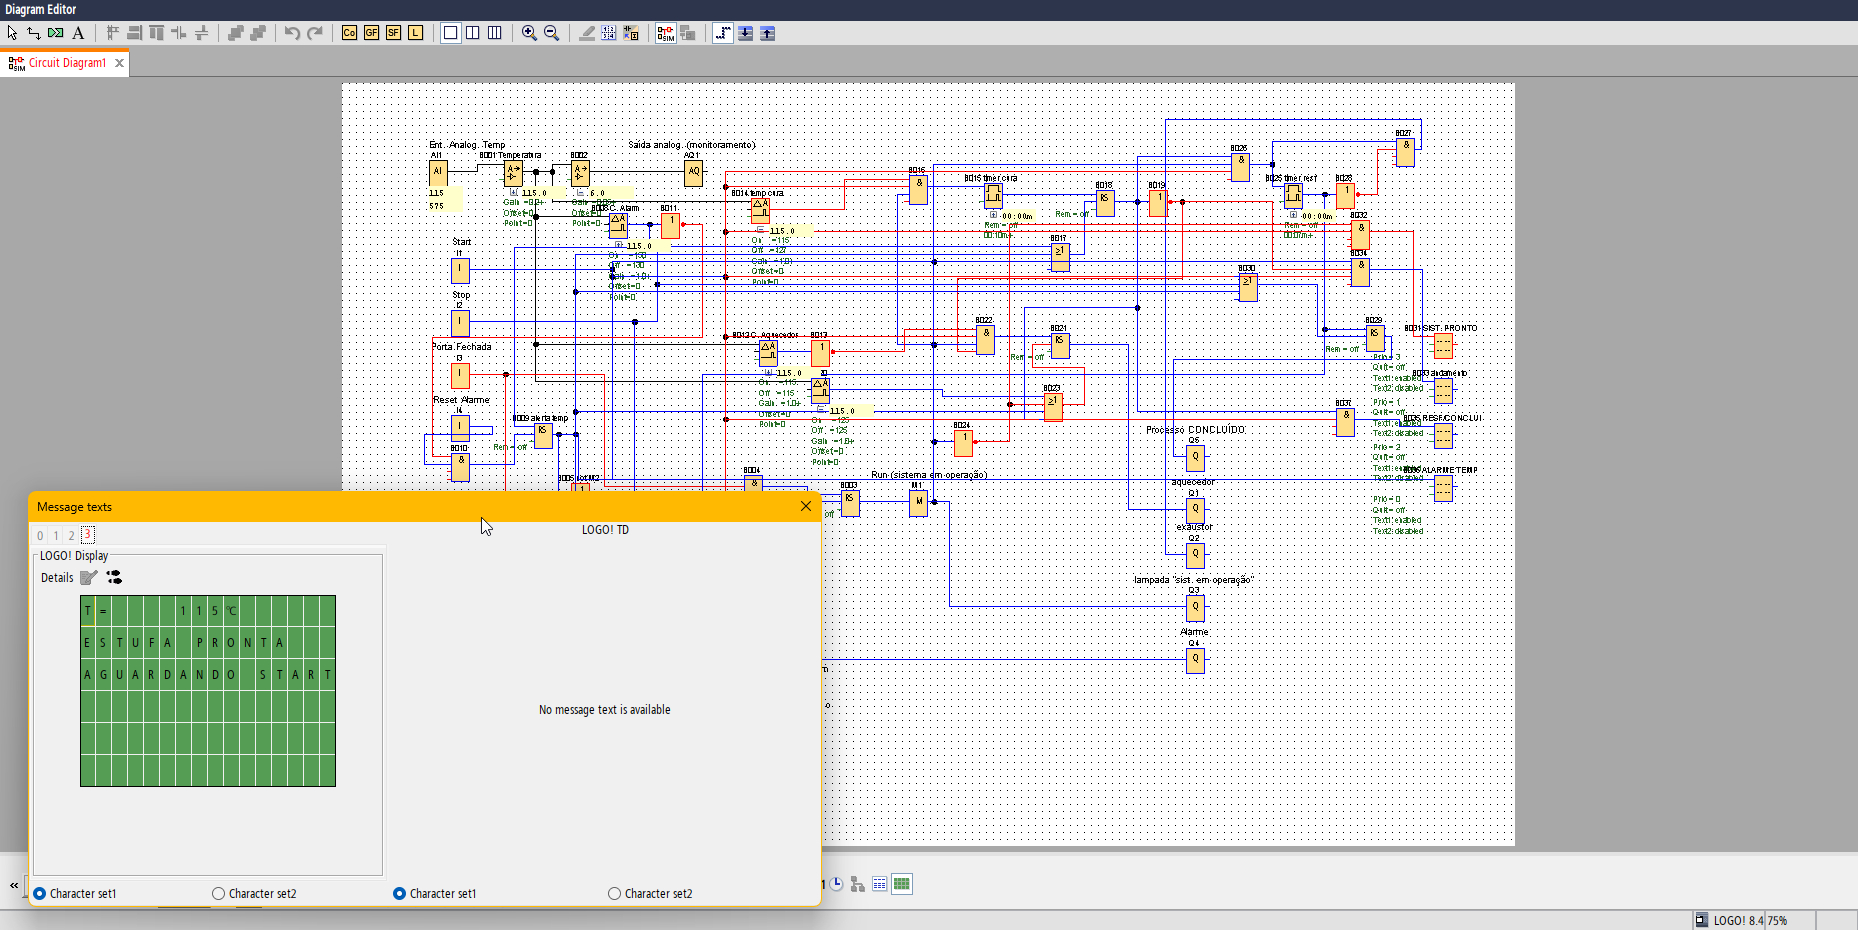
\includegraphics[width=1\textwidth]{IHM.png}
\caption{Tela da IHM no display do CLP LOGO! (Sistema Pronto).}
\label{fig:ihm_logo}
\end{figure}

\section{Implementa\c{c}\~{a}o no TPW-PCLINK (WEG)}

O mesmo algoritmo de controle foi implementado no CLP WEG TPW-04 utilizando o software TPW-PCLINK V1.12. A principal diferen\c{c}a em rela\c{c}\~{a}o ao LOGO! \'{e} a linguagem de programa\c{c}\~{a}o: enquanto o LOGO! utiliza exclusivamente FBD, o TPW-PCLINK permite a programa\c{c}\~{a}o em \textbf{Diagrama Ladder}, onde a l\'{o}gica \'{e} constru\'{i}da graficamente por meio de contatos, bobinas e blocos de fun\c{c}\~{a}o organizados em \textit{rungs}.

\subsection{Mapeamento de I/O no TPW-04}

O endere\c{c}amento no TPW-04 segue o padr\~{a}o da fam\'{i}lia: entradas digitais s\~{a}o designadas por X (numera\c{c}\~{a}o octal), sa\'{i}das por Y, mem\'{o}rias auxiliares por M, registradores de dados por D e temporizadores por T. O mapeamento completo est\'{a} apresentado na Tabela~\ref{tab:io_tpw}.

Para a simula\c{c}\~{a}o da entrada anal\'{o}gica de temperatura, foi utilizado um bloco MOV no diagrama Ladder para carregar um valor fixo no registrador D0 (por exemplo, o valor 600). O valor \'{e} ent\~{a}o dividido por 5 por um bloco DIV, resultando na temperatura em graus Celsius (600/5 = 120~\textdegree{}C). Em uma aplica\c{c}\~{a}o real, o bloco MOV seria substitu\'{i}do pela leitura de um m\'{o}dulo de expans\~{a}o anal\'{o}gica com a fun\c{c}\~{a}o EPSC (FNC~89) para escala autom\'{a}tica do sinal do sensor.

\subsection{Estrutura do Diagrama Ladder}

O programa Ladder desenvolvido no TPW-PCLINK \'{e} composto por 16 \textit{rungs} (degraus), cada qual respons\'{a}vel por uma fun\c{c}\~{a}o l\'{o}gica espec\'{i}fica. A seguir \'{e} apresentada a descri\c{c}\~{a}o de cada \textit{rung}:

\begin{itemize}
    \item \textbf{Rung 1 -- Leitura e escala de temperatura}: utiliza um contato sempre ligado (M8000) para acionar os blocos de fun\c{c}\~{a}o MOV (carrega o valor simulado em D0) e DIV (divide D0 por 5, armazenando o resultado em D1 como temperatura em \textdegree{}C).
    \item \textbf{Rung 2 -- Detec\c{c}\~{a}o de sobretemperatura}: um contato de compara\c{c}\~{a}o verifica se D1 $\geq$ 150; caso verdadeiro, uma bobina SET ativa a mem\'{o}ria M1 (alarme).
    \item \textbf{Rung 3 -- Reset de alarme}: o contato do bot\~{a}o Reset (X003) em s\'{e}rie com um contato de compara\c{c}\~{a}o (D1 $<$ 130) aciona uma bobina RST que desativa M1.
    \item \textbf{Rung 4 -- Sa\'{i}da de alarme}: o contato de M1 aciona a bobina Y003 (l\^{a}mpada/buzzer de alarme).
    \item \textbf{Rung 5 -- Partida do sistema}: contatos em s\'{e}rie de X000 (Start), X002 (porta fechada), M1 invertido (sem alarme) e M0 invertido (sistema parado) acionam bobinas SET para M0 (RUN) e RST para M3 e M4 (limpeza dos flags de cura e resfriamento).
    \item \textbf{Rung 6 -- Parada do sistema}: contatos de X001 (Stop), M1 (alarme), X002 invertido (porta aberta) e M4 (resfriamento completo) em paralelo acionam uma bobina RST que desativa M0.
    \item \textbf{Rung 7 -- L\^{a}mpada de opera\c{c}\~{a}o}: o contato de M0 aciona a bobina Y002.
    \item \textbf{Rung 8 -- Aquecedor ON (histerese inferior)}: um contato de compara\c{c}\~{a}o (D1 $<$ 115) em s\'{e}rie com M0, M1 invertido e M3 invertido aciona uma bobina SET para M2 (habilita aquecedor).
    \item \textbf{Rung 9 -- Aquecedor OFF (histerese superior)}: um contato de compara\c{c}\~{a}o (D1 $\geq$ 125) em paralelo com M1, M0 invertido e M3 aciona uma bobina RST para M2 (desabilita aquecedor).
    \item \textbf{Rung 10 -- Sa\'{i}da do aquecedor}: o contato de M2 aciona a bobina Y000 (contator do aquecedor).
    \item \textbf{Rung 11 -- Timer de cura}: contatos de compara\c{c}\~{a}o (D1 $\geq$ 115), M0, M1 invertido e M3 invertido acionam a bobina do temporizador T0 com \textit{setpoint} de 10~s para demonstra\c{c}\~{a}o (30~min em opera\c{c}\~{a}o real).
    \item \textbf{Rung 12 -- Cura completa}: o contato de T0 (timer expirado) aciona uma bobina SET para M3.
    \item \textbf{Rung 13 -- Timer de resfriamento}: contatos de M3, M0 e M4 invertido acionam a bobina do temporizador T1 com \textit{setpoint} de 7~s para demonstra\c{c}\~{a}o (5~min em opera\c{c}\~{a}o real).
    \item \textbf{Rung 14 -- Ventilador}: contatos de M3, M0 e M4 invertido acionam a bobina Y001 (ventilador).
    \item \textbf{Rung 15 -- Resfriamento completo}: o contato de T1 (timer expirado) aciona uma bobina SET para M4.
    \item \textbf{Rung 16 -- Processo conclu\'{i}do}: o contato de M4 aciona a bobina Y004 (l\^{a}mpada ``conclu\'{i}do'').
\end{itemize}

As Figuras~\ref{fig:tpw_ladder1} e~\ref{fig:tpw_ladder2} apresentam o Diagrama Ladder desenvolvido no TPW-PCLINK.

\begin{figure}[ht!]
\centering
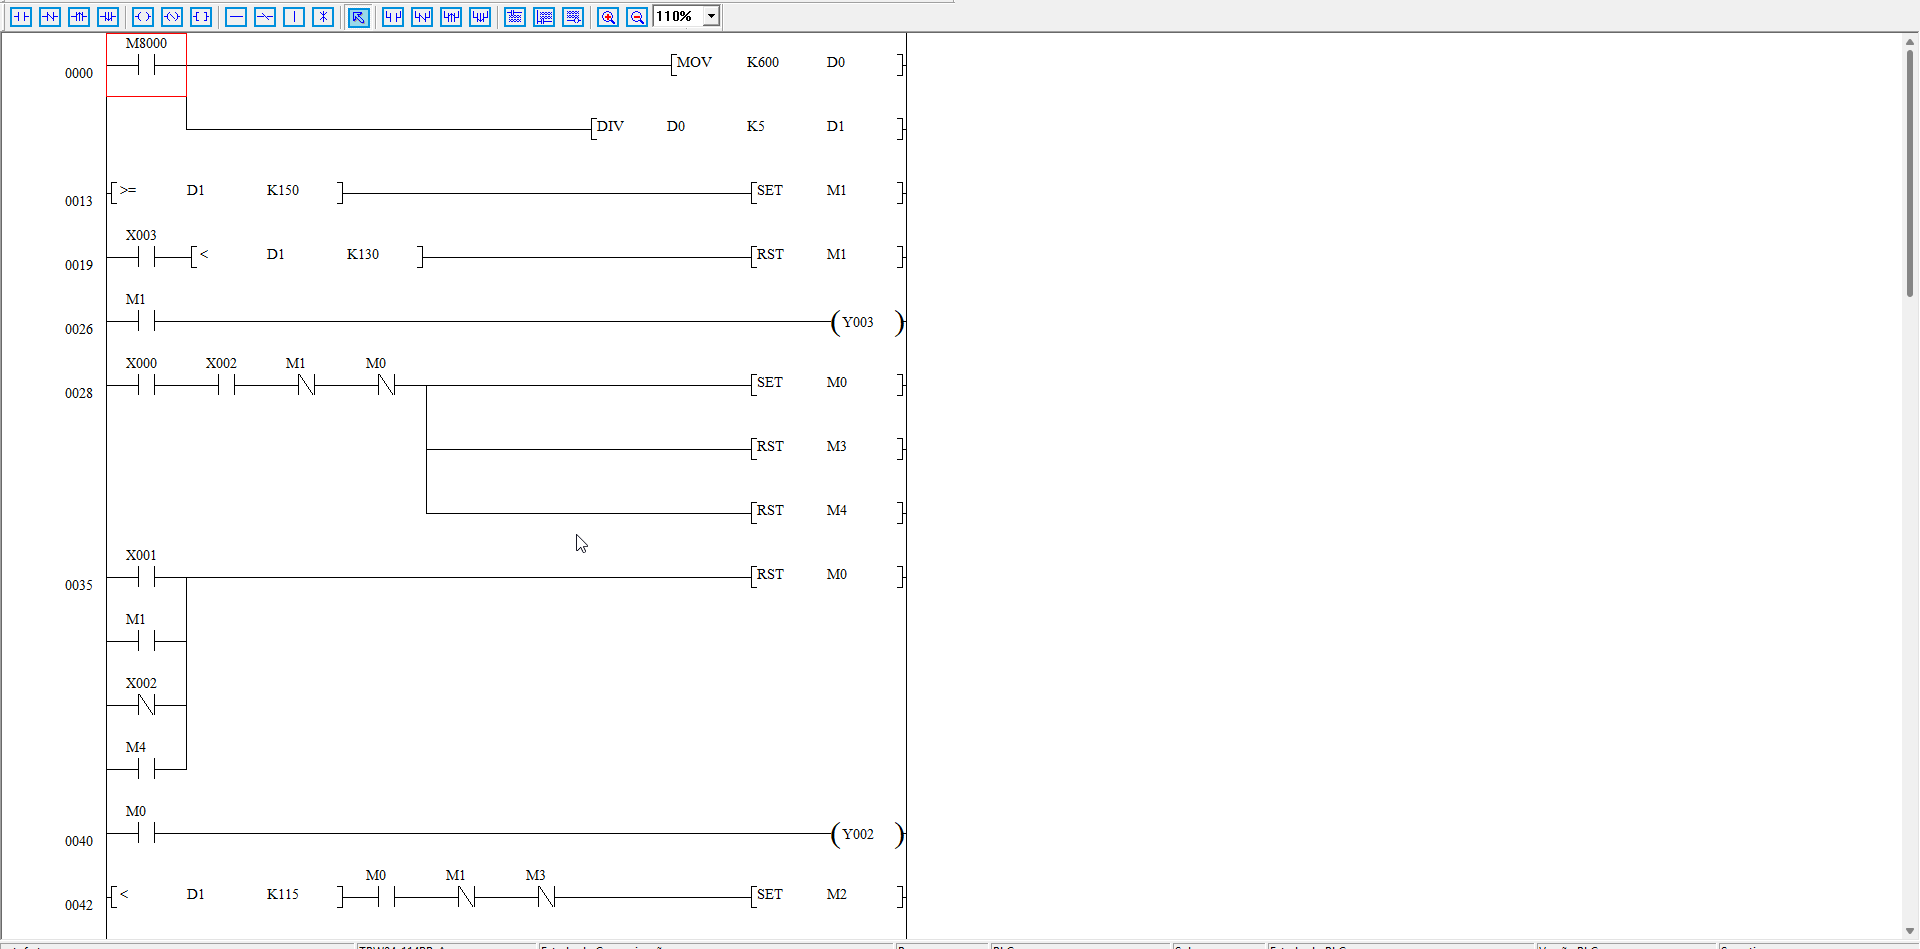
\includegraphics[width=1\textwidth]{tpw_ladder1.png}
\caption{Diagrama Ladder no TPW-PCLINK -- parte superior (Rungs 1 a 10).}
\label{fig:tpw_ladder1}
\end{figure}

\begin{figure}[ht!]
\centering
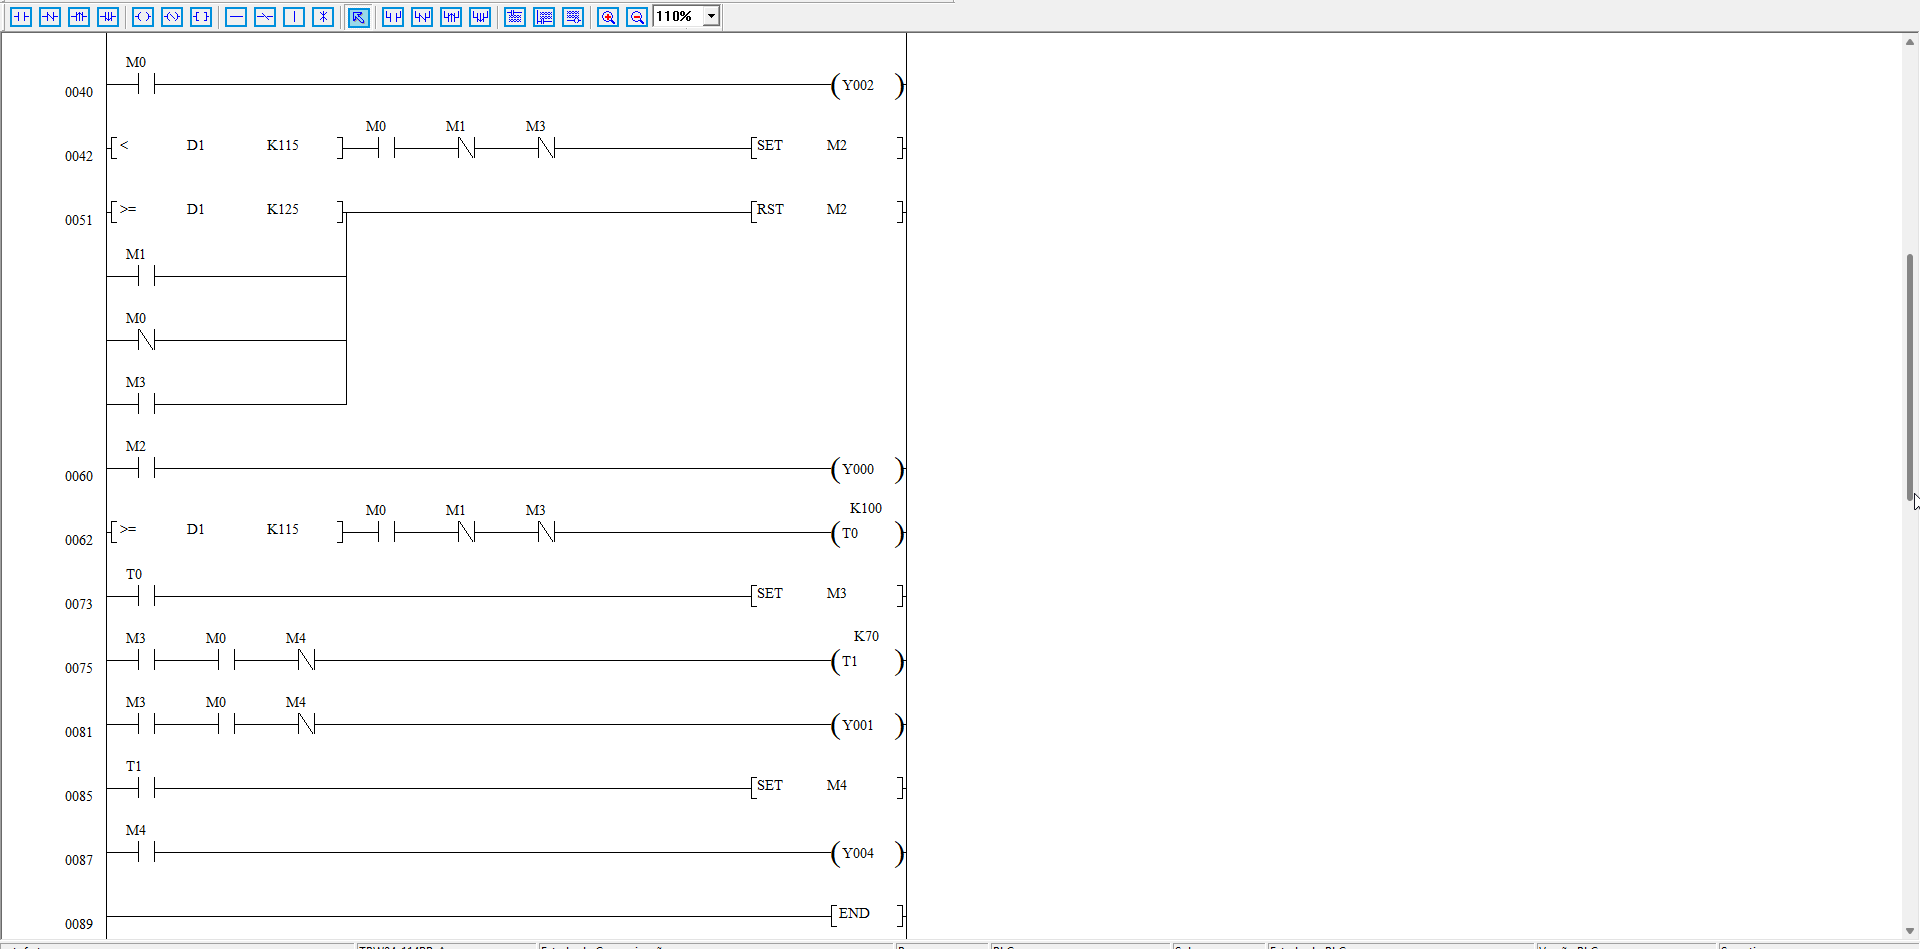
\includegraphics[width=1\textwidth]{tpw_ladder2.png}
\caption{Diagrama Ladder no TPW-PCLINK -- parte inferior (Rungs 11 a 16 e END).}
\label{fig:tpw_ladder2}
\end{figure}

\clearpage

\subsection{Descri\c{c}\~{a}o das l\'{o}gicas por \textit{rung}}

A Tabela~\ref{tab:rungs} apresenta um resumo da fun\c{c}\~{a}o de cada \textit{rung} do programa no TPW-04 e a correspond\^{e}ncia com os blocos do LOGO!.

\begin{table}[htbp]
\centering
\caption{Correspond\^{e}ncia entre \textit{rungs} do TPW-04 e blocos do LOGO!.}
\label{tab:rungs}
\small
\begin{tabular}{clll}
\toprule
\textbf{Rung} & \textbf{Fun\c{c}\~{a}o} & \textbf{TPW-04} & \textbf{LOGO!} \\
\midrule
1  & Leitura de temperatura    & Blocos MOV + DIV         & Amplif. anal\'{o}gico B001 \\
2  & Sobretemperatura (SET)    & Compara\c{c}\~{a}o ($\geq$150) + bobina SET M1  & Comparador B014 + RS \\
3  & Reset alarme              & Contato X003 + compara\c{c}\~{a}o ($<$130) + bobina RST & Comparador B015 + I4 \\
4  & Sa\'{i}da alarme               & Bobina Y003         & Q4 \\
5  & Partida (SET RUN)         & Bobina SET M0           & RS (RUN) -- Set \\
6  & Parada (RST RUN)          & Bobina RST M0           & RS (RUN) -- Reset \\
7  & L\^{a}mpada opera\c{c}\~{a}o          & Bobina Y002         & Q3 \\
8  & Aquecedor ON              & Compara\c{c}\~{a}o ($<$115) + bobina SET M2   & Comparador B003 + RS \\
9  & Aquecedor OFF             & Compara\c{c}\~{a}o ($\geq$125) + bobina RST M2  & Comparador B013 + RS \\
10 & Sa\'{i}da aquecedor            & Bobina Y000         & Q1 \\
11 & Timer de cura             & Bobina temporizador T0  & Temporizador \textit{on-delay} \\
12 & Cura completa             & Bobina SET M3           & RS (cura finalizada) \\
13 & Timer resfriamento        & Bobina temporizador T1  & Temporizador \textit{on-delay} \\
14 & Ventilador                & Bobina Y001         & Q2 \\
15 & Resfriamento completo     & Bobina SET M4           & RS (resfriamento) \\
16 & Processo conclu\'{i}do         & Bobina Y004         & Q5 \\
\bottomrule
\end{tabular}
\end{table}

\clearpage
\section{Compara\c{c}\~{a}o entre as plataformas}

A Tabela~\ref{tab:comparacao} apresenta uma compara\c{c}\~{a}o t\'{e}cnica entre as duas plataformas utilizadas neste projeto.

\begin{table}[htbp]
\centering
\caption{Compara\c{c}\~{a}o entre Siemens LOGO! e WEG TPW-04.}
\label{tab:comparacao}
\small
\begin{tabular}{p{4cm}p{5cm}p{5cm}}
\toprule
\textbf{Caracter\'{i}stica} & \textbf{Siemens LOGO!} & \textbf{WEG TPW-04} \\
\midrule
Linguagem de programa\c{c}\~{a}o & FBD (Diagrama de Blocos Funcionais) & Ladder (LD) \\
\addlinespace
Software & LOGO!Soft Comfort & TPW-PCLINK V1.12 \\
\addlinespace
Formato do projeto & .lsc & .tpc \\
\addlinespace
Entrada anal\'{o}gica & Integrada (AI1--AI8, 0--10~V) & Via expans\~{a}o anal\'{o}gica ou simula\c{c}\~{a}o por registrador \\
\addlinespace
Sa\'{i}da anal\'{o}gica & Integrada (AQ1--AQ2) & Via expans\~{a}o anal\'{o}gica \\
\addlinespace
Endere\c{c}amento de I/O & Decimal (I1, Q1) & Octal (X000, Y000) \\
\addlinespace
Flip-flop RS & Bloco RS dedicado & Bobinas SET/RST \\
\addlinespace
Compara\c{c}\~{a}o anal\'{o}gica & Bloco comparador com limiares & Contatos de compara\c{c}\~{a}o no Ladder \\
\addlinespace
Escala anal\'{o}gica & Bloco amplificador (ganho + offset) & Blocos de fun\c{c}\~{o}es aritm\'{e}ticas (MUL, DIV) \\
\addlinespace
Temporizadores & Blocos \textit{on-delay} com par\^{a}metros & T0--T255 com base de tempo fixa \\
\addlinespace
Display/IHM & Display integrado com blocos de texto & N\~{a}o dispon\'{i}vel (requer IHM externa) \\
\addlinespace
Capacidade de programa & $\sim$400 blocos & At\'{e} 8000 passos \\
\addlinespace
PID integrado & N\~{a}o dispon\'{i}vel no modelo b\'{a}sico & FNC~88 (PID completo) \\
\addlinespace
Comunica\c{c}\~{a}o & Ethernet (modelos RCE) & RS485, MODBUS RTU/ASCII \\
\bottomrule
\end{tabular}
\end{table}

%% ============================================================
\chapter{Resultados e discuss\~{a}o}
%% ============================================================

\section{Resultados da implementa\c{c}\~{a}o no LOGO!}

O programa desenvolvido no LOGO!Soft Comfort foi validado em simula\c{c}\~{a}o, apresentando o comportamento esperado em todas as condi\c{c}\~{o}es testadas. Ao acionar o bot\~{a}o \textit{Start} com a porta fechada e sem alarmes, o sistema entra em opera\c{c}\~{a}o, liga o aquecedor e a temperatura come\c{c}a a subir. Ao atingir a faixa de histerese (115--125~\textdegree{}C), o aquecedor passa a alternar entre ligado e desligado, mantendo a temperatura em torno do \textit{setpoint} de 120~\textdegree{}C.

Quando a temperatura entra na faixa de cura, o temporizador \'{e} iniciado. Ao fim do per\'{i}odo de cura, o aquecedor \'{e} bloqueado e o ventilador \'{e} acionado para resfriamento. Ap\'{o}s o resfriamento, o sistema retorna ao estado de espera com indica\c{c}\~{a}o de processo conclu\'{i}do.

A detec\c{c}\~{a}o de sobretemperatura e o intertravamento de porta funcionaram corretamente, desligando o aquecedor e acionando o alarme nas condi\c{c}\~{o}es de falha, com necessidade de \textit{reset} manual para retomada da opera\c{c}\~{a}o.

\section{Resultados da implementa\c{c}\~{a}o no TPW-04}

O programa em Diagrama Ladder desenvolvido para o TPW-04 implementa a mesma l\'{o}gica de controle do LOGO!, por\'{e}m utilizando contatos, bobinas e blocos de fun\c{c}\~{a}o organizados em \textit{rungs}. A utiliza\c{c}\~{a}o do bloco MOV para carregar valores fixos no registrador D0 permitiu simular diferentes condi\c{c}\~{o}es de temperatura e testar todas as faixas de opera\c{c}\~{a}o.

O programa possui 16 \textit{rungs} l\'{o}gicos, cada qual com fun\c{c}\~{a}o bem definida, e utiliza 5 mem\'{o}rias auxiliares (M0--M4), 2 temporizadores (T0--T1) e 2 registradores de dados (D0--D1). A l\'{o}gica de histerese \'{e} implementada por pares de bobinas SET/RST condicionadas por contatos de compara\c{c}\~{a}o, o que equivale funcionalmente aos blocos RS com comparadores do LOGO!.

\clearpage
\section{An\'{a}lise comparativa}

A implementa\c{c}\~{a}o dual evidenciou as seguintes observa\c{c}\~{o}es:

\begin{itemize}
    \item \textbf{Abordagem de programa\c{c}\~{a}o}: o LOGO! favorece uma abordagem visual e intuitiva, com blocos sendo conectados graficamente. O TPW-04, atrav\'{e}s do Diagrama Ladder, tamb\'{e}m utiliza uma abordagem gr\'{a}fica, por\'{e}m baseada na l\'{o}gica de rel\'{e}s, com contatos e bobinas organizados em degraus, o que facilita a interpreta\c{c}\~{a}o por profissionais familiarizados com circuitos el\'{e}tricos.
    \item \textbf{Tratamento anal\'{o}gico}: no LOGO!, blocos dedicados (amplificador e comparador) simplificam o processamento de sinais anal\'{o}gicos. No TPW-04, a mesma funcionalidade requer blocos de fun\c{c}\~{o}es aritm\'{e}ticas e contatos de compara\c{c}\~{a}o, oferecendo maior flexibilidade mas exigindo mais conhecimento do programador.
    \item \textbf{Mem\'{o}ria e reten\c{c}\~{a}o}: ambos os CLPs suportam l\'{o}gicas de reten\c{c}\~{a}o (RS/SET-RST), por\'{e}m com sintaxes distintas. No LOGO!, o bloco RS \'{e} um elemento gr\'{a}fico com entradas Set e Reset. No TPW-04, as bobinas SET e RST atuam sobre o mesmo endere\c{c}o de mem\'{o}ria, sendo que a \'{u}ltima bobina executada no ciclo de varredura determina o estado final.
    \item \textbf{IHM}: o LOGO! possui display integrado, permitindo a implementa\c{c}\~{a}o de interfaces simples sem hardware adicional. O TPW-04 n\~{a}o possui display, necessitando de IHM externa para monitoramento visual.
    \item \textbf{Recursos avan\c{c}ados}: o TPW-04 oferece recursos n\~{a}o dispon\'{i}veis no LOGO! b\'{a}sico, como controle PID integrado, opera\c{c}\~{o}es em ponto flutuante, fun\c{c}\~{o}es trigonom\'{e}tricas e comunica\c{c}\~{a}o MODBUS, que seriam vantajosos em aplica\c{c}\~{o}es mais complexas.
\end{itemize}

Como limita\c{c}\~{a}o, ressalta-se que o controle de temperatura implementado em ambas as plataformas \'{e} do tipo liga/desliga, o que, embora seja adequado para muitos processos de secagem, n\~{a}o apresenta a mesma precis\~{a}o de um controle PID. Em aplica\c{c}\~{o}es mais exigentes, o TPW-04 ofereceria vantagem ao possibilitar a implementa\c{c}\~{a}o de controle PID nativo (FNC~88).

%% ============================================================
\chapter{Conclus\~{a}o}
%% ============================================================

Este trabalho apresentou o desenvolvimento de um sistema de controle de temperatura para uma estufa de secagem utilizada na cura de tinta em pe\c{c}as met\'{a}licas, implementado em duas plataformas de CLP: Siemens LOGO! (programado em FBD) e WEG TPW-04 (programado em Ladder).

Os objetivos foram alcan\c{c}ados, uma vez que ambas as implementa\c{c}\~{o}es s\~{a}o capazes de:

\begin{itemize}
    \item monitorar a temperatura interna da estufa;
    \item controlar o aquecedor de forma autom\'{a}tica, utilizando l\'{o}gica liga/desliga com histerese para manter a temperatura em torno do \textit{setpoint} de cura;
    \item realizar o tempo de cura das pe\c{c}as dentro da faixa adequada de temperatura;
    \item promover o resfriamento controlado da estufa ap\'{o}s a cura;
    \item garantir seguran\c{c}a por meio de detec\c{c}\~{a}o de sobretemperatura, alarme e bloqueio de opera\c{c}\~{a}o, bem como intertravamento de porta.
\end{itemize}

A implementa\c{c}\~{a}o dual permitiu comparar as caracter\'{i}sticas de duas plataformas de CLP amplamente utilizadas na ind\'{u}stria brasileira, evidenciando que o mesmo algoritmo de controle pode ser traduzido para diferentes linguagens e ambientes de programa\c{c}\~{a}o. A experi\^{e}ncia de programar o mesmo projeto em FBD (LOGO!) e Ladder (TPW-04) consolidou o dom\'{i}nio de conceitos fundamentais como endere\c{c}amento de I/O, l\'{o}gica de reten\c{c}\~{a}o, temporiza\c{c}\~{a}o, tratamento de sinais anal\'{o}gicos e intertravamentos de seguran\c{c}a.

Do ponto de vista did\'{a}tico, o projeto demonstrou que a escolha da plataforma de CLP depende dos requisitos da aplica\c{c}\~{a}o, dos recursos necess\'{a}rios e da prefer\^{e}ncia do programador pela linguagem de programa\c{c}\~{a}o. Enquanto o LOGO! se destaca pela facilidade de programa\c{c}\~{a}o visual e pela IHM integrada, o TPW-04 oferece maior capacidade computacional e recursos avan\c{c}ados como PID e MODBUS.

% Referencias
\postextual

\renewcommand{\bibsection}{%
  \chapter*{REFER\^{E}NCIAS}
  \addcontentsline{toc}{chapter}{REFER\^{E}NCIAS}
}

\begin{thebibliography}{99}

\bibitem{aulas-clp}
PEREIRA, V. M.
\textbf{Notas de aula da disciplina de Controladores L\'{o}gicos Program\'{a}veis}.
Campo Grande: UFMS, 2025.

\bibitem{logo-manual}
SIEMENS.
\textbf{LOGO!}: manual do produto. 6. ed. Nuremberga: Siemens AG, 2014. Dispon\'{i}vel em: \url{https://www.siemens.com}. Acesso em: 10 maio 2025.

\bibitem{tpw-manual}
WEG.
\textbf{Controlador program\'{a}vel TPW-04}: manual de programa\c{c}\~{a}o. Jaragu\'{a} do Sul: WEG Equipamentos El\'{e}tricos, 2020.

\bibitem{iec61131}
INTERNATIONAL ELECTROTECHNICAL COMMISSION.
\textbf{IEC 61131-3}: programmable controllers -- part 3: programming languages. 3. ed. Geneva: IEC, 2013.

\end{thebibliography}

\end{document}
